\documentclass[a4paper,11pt]{article}
% Various packages
\usepackage{siunitx}
\usepackage[utf8]{inputenc} % æøå
\usepackage[T1]{fontenc} % mere æøå
\usepackage[danish]{babel} % orddeling
\usepackage{verbatim} % så man kan skrive ren tekst
\usepackage{graphicx}
\graphicspath{{assets/}}
\usepackage{a4wide}
\usepackage{url}
\usepackage[left=2cm,top=2cm,bottom=1.5cm,right=2cm]{geometry}
\usepackage{amsmath}
\usepackage{amssymb}
\usepackage{amsthm}
\usepackage{wrapfig}
\usepackage{fixme}
\usepackage{color}
\usepackage{pstricks}
\usepackage{pdfpages} % include pdf
\usepackage{float} % Use [H] in figures
\usepackage{subcaption} % For subfigures
\usepackage{color} % May be necessary if you want to color links
\usepackage{hyperref} % Make references clickable
\usepackage[nameinlink,capitalize]{cleveref} % Make eq:refs be in style (1)
\usepackage[linesnumbered, commentsnumbered, lined, ruled, vlined,
%noend  % Have no ⌊-like symbol to indicate end of scope in pseudocode
]{algorithm2e} % Doc: https://goo.gl/6bC1qZ

% Ændr på navnene der vises når man bruger \autoref{label}
\def\sectionautorefname{Sektion}
\renewcommand{\equationautorefname}{Ligning}
\def\figureautorefname{Figur}
\AtBeginDocument{\renewcommand{\ref}[1]{\autoref{#1}}}

% Sæt \ref{} til at kalde \autoref{}
\AtBeginDocument{\renewcommand{\ref}[1]{\autoref{#1}}}

% Ændr ''*'' i math-felter til \cdot
\DeclareMathSymbol{*}{\mathbin}{symbols}{"01}

% Sæt farver for interne referencer og links
\definecolor{darkblue}{RGB}{25,25,112}
\hypersetup{
	colorlinks=true,    %set true if you want colored links
	linktoc=all,        %set to all if you want both sections and subsections linked
	linkcolor=darkblue, %choose some color if you want links to stand out
	filecolor=blue,     %
	citecolor=black,    %
	urlcolor=cyan,      %
}

% Set indentation to 0:
\setlength\parindent{0pt}

% Keywords relateret til algorithm2e pakken
\newcommand{\True}{\textbf{true}}\newcommand{\False}{\textbf{false}}
\SetStartEndCondition{ }{}{}%
\SetKwProg{Fn}{def}{\string:}{}
\SetKw{KwTo}{to}
\SetKwFor{For}{for}{}{}% 
\SetKwFor{ForEach}{foreach}{}{}% 
\SetKwIF{If}{ElseIf}{Else}{if}{}{elif}{else}{end}% 
\SetKwFor{While}{while}{}{end}\SetKwProg{Fn}{}{}{}
\SetKwInOut{Input}{input}\SetKwInOut{Output}{output}
\setlength{\algomargin}{3em}\DontPrintSemicolon

\newcommand{\longspace}{{\ \ \ \ \ \ \ \ \ \ \ \ \ \ }}
\renewcommand{\P}{{\mathbb P}}
\newcommand{\parfrac}[1]{\frac{\partial}{\partial #1}}
\renewcommand{\num}{{\textrm{num} }}
\newcommand{\size}{{\textrm{size} }}
\newcommand{\ift}{{\textrm{if } }}

% Dynamiske (), <>, ceil, floor
\newcommand{\p}[1]{\left( #1 \right)}
\newcommand{\pbig}[1]{\big( #1 \big)}
\newcommand{\pBig}[1]{\Big( #1 \Big)}
\newcommand{\pbigg}[1]{\bigg( #1 \bigg)}
\newcommand{\larr}[1]{\left< #1 \right>}
\newcommand{\ceil}[1]{\left\lceil #1 \right\rceil}
\newcommand{\floor}[1]{\left\lfloor #1 \right\rfloor}


% Squiggly arrows
\DeclareFontFamily{U} {MnSymbolC}{}

\DeclareFontShape{U}{MnSymbolC}{m}{n}{
	<-6> MnSymbolC5
	<6-7> MnSymbolC6
	<7-8> MnSymbolC7
	<8-9> MnSymbolC8
	<9-10> MnSymbolC9
	<10-12> MnSymbolC10
	<12-> MnSymbolC12}{}
\DeclareFontShape{U}{MnSymbolC}{b}{n}{
	<-6> MnSymbolC-Bold5
	<6-7> MnSymbolC-Bold6
	<7-8> MnSymbolC-Bold7
	<8-9> MnSymbolC-Bold8
	<9-10> MnSymbolC-Bold9
	<10-12> MnSymbolC-Bold10
	<12-> MnSymbolC-Bold12}{}

\DeclareSymbolFont{MnSyC} {U} {MnSymbolC}{m}{n}

\DeclareMathSymbol{\MNrhd}{\mathbin}{MnSyC}{76}
\DeclareMathSymbol{\MNlhd}{\mathbin}{MnSyC}{78}
% =============================================
\DeclareFontFamily{U} {MnSymbolD}{}

\DeclareFontShape{U}{MnSymbolD}{m}{n}{
	<-6> MnSymbolD5
	<6-7> MnSymbolD6
	<7-8> MnSymbolD7
	<8-9> MnSymbolD8
	<9-10> MnSymbolD9
	<10-12> MnSymbolD10
	<12-> MnSymbolD12}{}
\DeclareFontShape{U}{MnSymbolD}{b}{n}{
	<-6> MnSymbolD-Bold5
	<6-7> MnSymbolD-Bold6
	<7-8> MnSymbolD-Bold7
	<8-9> MnSymbolD-Bold8
	<9-10> MnSymbolD-Bold9
	<10-12> MnSymbolD-Bold10
	<12-> MnSymbolD-Bold12}{}

\DeclareSymbolFont{MnSyD} {U} {MnSymbolD}{m}{n}
\DeclareMathSymbol{\MNsim}{\mathbin}{MnSyD}{2}

% =============================================

\usepackage{amssymb,amsmath,stackengine}
\stackMath
\newcommand\rsquigarrow[1]{%
	\mathbin{\stackon[2pt]{\rightsquigarrow}{\scriptscriptstyle #1 }}
}

\author{Søren Mulvad, rbn601}

\title{Eksamensdisposition - Del og hersk}

\begin{document}
\maketitle

% Desuden skal hver studerende i gruppen udarbejde en individuel disposition for emnet "Divide and Conquer", som er et af emnerne til eksamen. En disposition skal bestå af de vigtigste punkter, du vil komme ind på til eksamen.
% Tænk på dispositionen som noget, du kan have med dig til eksamen, og som kan hjælpe dig med at huske, hvad du overordnet vil gennemgå til emnet "Divide and Conquer".
% Dispositionen skal ikke indeholde detaljerede beviser og lignende, men de mere overordnede delemner. Sørg for at gøre den kortfattet - f.eks. 5-10 punkter med stikord/-sætninger.


\begin{itemize}
	\item \textbf{Paradigmet}
	\item \textbf{Håndkørsel af \texttt{MergeSort}}
	\item \textbf{Rekursionsrelationer}
	\begin{itemize}
		\item Rekursionstræer
		\item Substitutionsmetoden
		\item Kort om Mastermetoden
	\end{itemize}
	\item \textbf{Bevis for lower bound for sortering}
\end{itemize}




%%%%%%%%%%%%%%%%%%%%%%%%%%%%%%%%%%%%%%%%%%%%%%%%%%%%%%%%%%%
%%%%%%%%%%%%%%%%%%%%%%%%%%%%%%%%%%%%%%%%%%%%%%%%%%%%%%%%%%%
%%%%%%%%%%%%%%%%%%%%%%%%%%%%%%%%%%%%%%%%%%%%%%%%%%%%%%%%%%%
\newpage
%%%%%%%%%%%%%%%%%%%%%%%%%%%%%%%%%%%%%%%%%%%%%%%%%%%%%%%%%%%
%%%%%%%%%%%%%%%%%%%%%%%%%%%%%%%%%%%%%%%%%%%%%%%%%%%%%%%%%%%
%%%%%%%%%%%%%%%%%%%%%%%%%%%%%%%%%%%%%%%%%%%%%%%%%%%%%%%%%%%
\section{Divide and Conquer (Del-og-hersk)}


\begin{itemize}
\item \textbf{Paradigmet} 
\begin{itemize}
	\item \textit{Del} problemet ind i en mængde af delproblemer som er mindre instanser af det samme problem.
	\item \textit{Hersk} (løs) delproblemerne ved at løse dem rekursivt. Hvis delproblemerne er tilpas små, så løs dem bare ''direkte''.
	\item \textit{Kombinér} løsningerne til delproblemerne sammen til én løsning til det oprindelige problem.
	\item Minder en smule om Dynamisk Programmering, men forskellen er, at problemerne ikke har optimal delstruktur, altså der er ikke overlappende delproblemer.
	\item Eksempler på algoritmer der benytter det er \texttt{QuickSort}, \texttt{Find-Maximum-Subarray} og \texttt{MergeSort}, som jeg vil gå mere i dybden med nu.
\end{itemize}


\item \textbf{Håndkørsel af \texttt{MergeSort}}
\begin{figure}[H]
	\begin{center}
		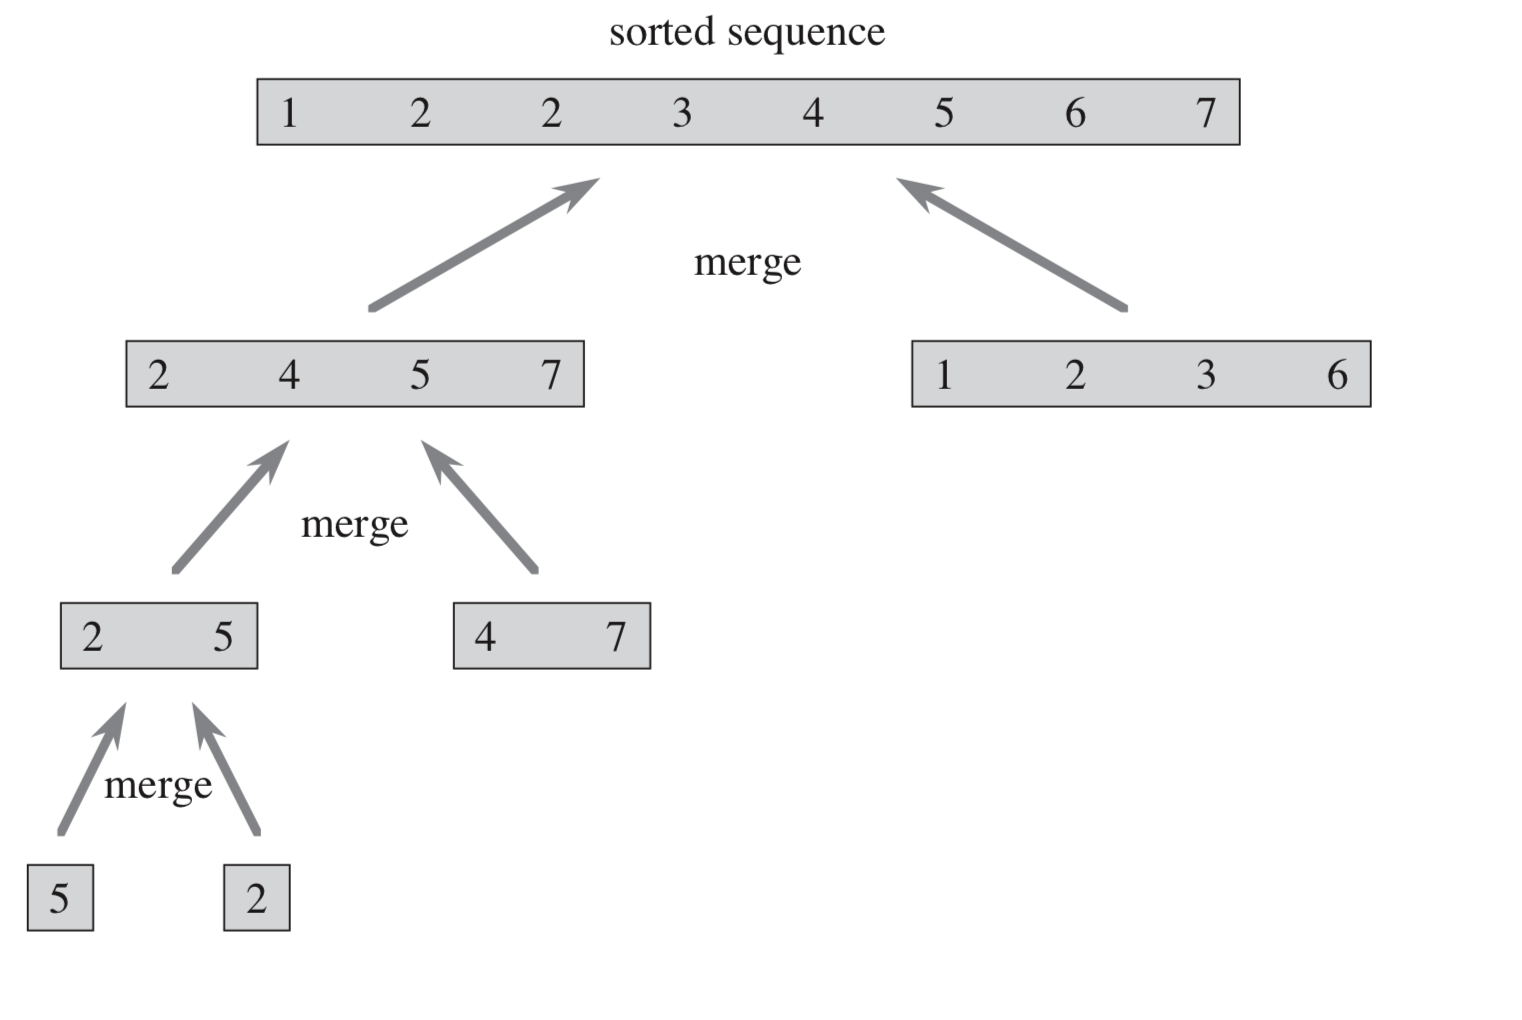
\includegraphics[width=0.8\textwidth]{merge.png}
	\end{center}
	\caption{Tegn et træ ala dette, hvor du så kun viser ned i venstre side. Sørg for at holde det 8 elementer langt.}
	\label{fig:merge}
\end{figure}
Jeg vil vise det på en 2-talspotens, for det gør det lidt nemmere at illustrere, men princippet ville være det samme for andre tal. Del arrayet op i to (ca.) lige store dele, kald \texttt{Merge-Sort} på disse og \texttt{Merge} til sidst de nu sorterede delarrays. Algoritmen kører i $O(n \lg n)$ tid, og det vil jeg nu bevise.


\item \textbf{Rekursionsrelationer}\\
Rekursionsrelationer er de typer relationer vi typisk vil få ved del og hersk algoritmer. Som et eksempel ses her rekursionsrelationen for \texttt{MergeSort}, hvor vi undlader at skrive casen når $n = 1$ eksplicit og ignorer, at vi egentlig skal tage floor og ceiling, altså tager udgangspunkt i den case hvor vi har en 2-talspotens. Vi får denne rekursionsrelation, da vi åbner to nye delproblemer der er af halv størrelse af det originale, og derudover til sidst skal samle det originale:
$$
T(n) = 2 T(n/2) + cn
$$



\item \textbf{Rekursionstræer}\\
Kan, hvis man er meget præcis, bruges til at bevise en rekursionsrelation. Bruges dog oftest til at komme på et godt gæt man så kan bevise med substitutionsmetoden. Her ses rekursionstræet vi får for \texttt{MergeSort} idet vi bruger ovenstående rekursionsrelation:
\begin{figure}[H]
	\begin{center}
		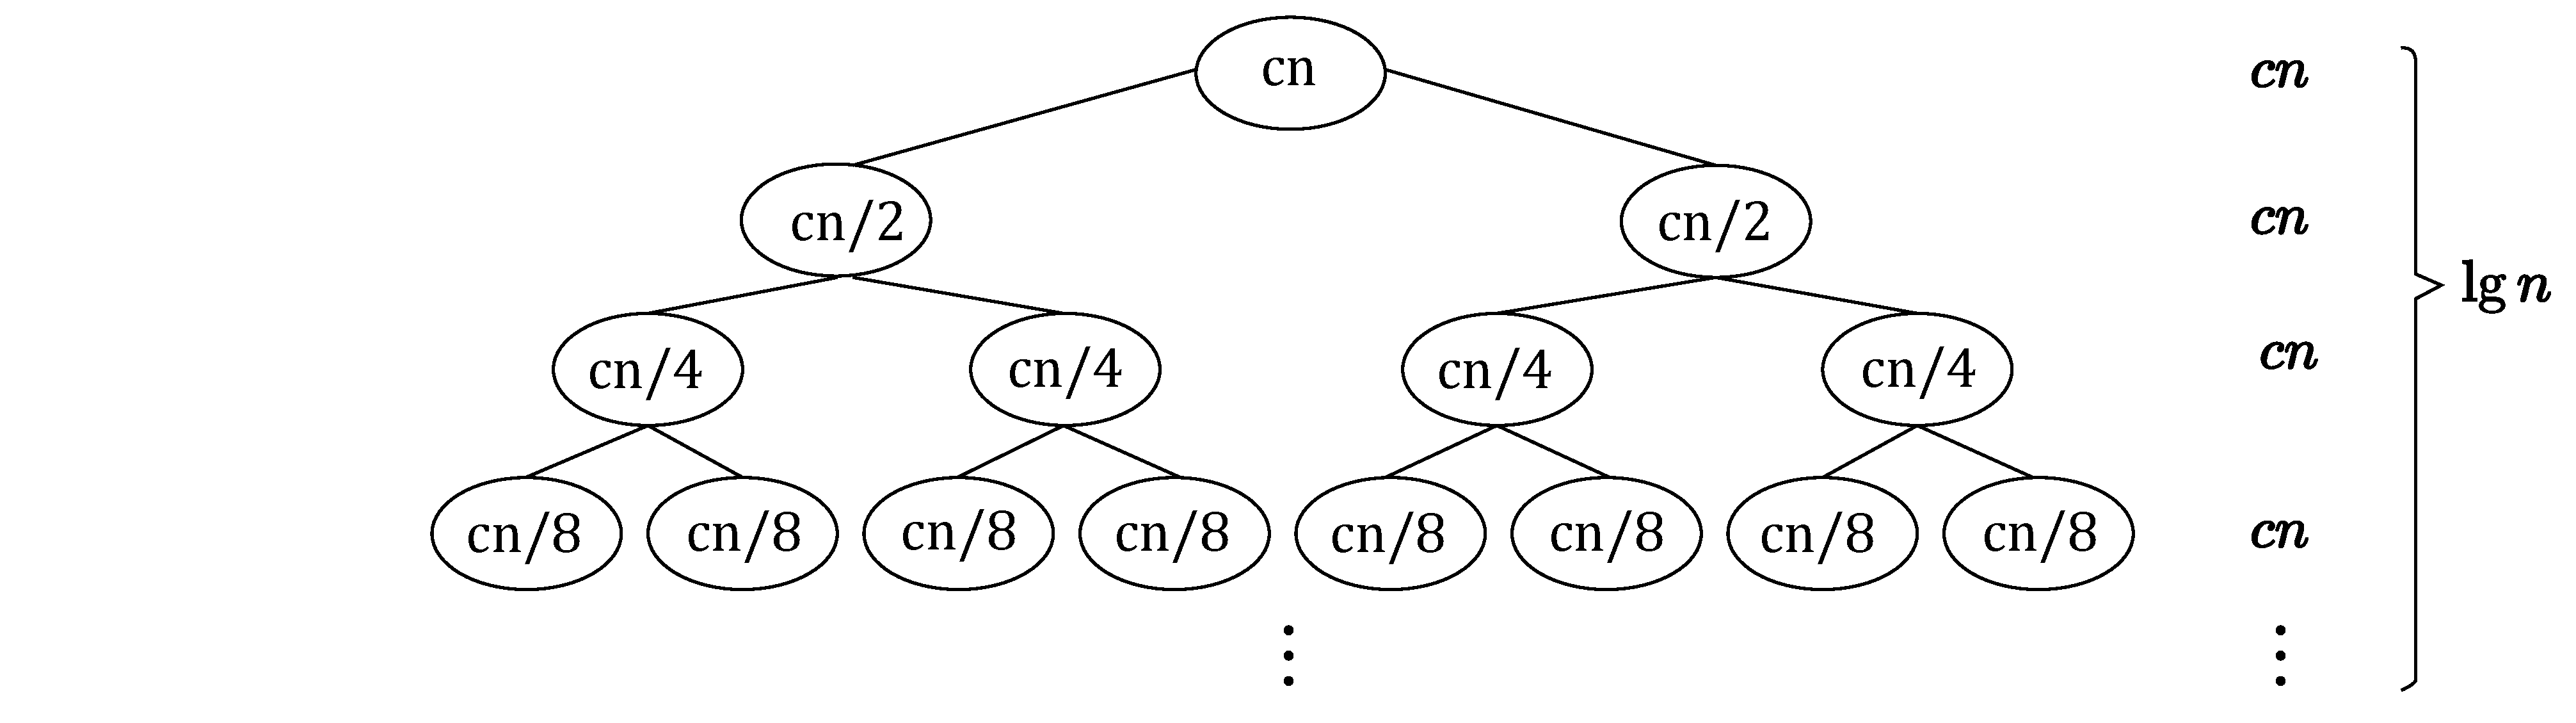
\includegraphics[width=\textwidth]{rectree.pdf}
	\end{center}
	\caption{Rekursionstræ for \texttt{MergeSort}}
	\label{fig:tree}
\end{figure}

Vi ser, at hvert niveau i træet bidrager med $cn$ og der er $\lg n$ af disse led. Derfor gætter vi på, at køretiden af \texttt{MergeSort} er $O(n \lg n)$. Vi gætter på dette:
$$
T(n) = 2 T(n/2) + n \quad\quad \text{har køretid} \quad\quad O(n \lg n)
$$

\item \textbf{Substitutionsmetoden}
\begin{enumerate}
	\item Gæt på en løsning (enten ud fra erfaring eller ved at tegne et rekursionstræ)
	\item Bevis din løsning er sand ved hjælp af induktion (OBS: Vær opmærksom på vi ikke kan være så ligeglad med konstanter som vi ellers tit er med O-notation). Hvis vi løber ind i et problem kan det ofte være en hjælp at trække et led af en lavere orden fra.
	\item Hvis du stadig ikke kan bevise det, så lav et nyt gæt og prøv igen.
\end{enumerate}

Til dette bevis skulle vi normalt bruge stærk induktion, men da vi antager det er en 2-talspotens er det ikke nødvendigt.\\

\textit{Base case:}\\
Vi skal nu vise $T(n) \leq cn \lg n$, hvor vi antager $T(1) = 1$. Vi ser, at vi ikke kan vise det for $n = 1$ da vi så får $cn \lg n = 0$ da $\lg 1 = 0$.

For $n = 2$:
$$
T(2) = 2T(\floor{2/2}) + 2 = 2T(1) + 2 = 4 \leq c 2 = c 2 \lg 2
$$
Hvilket er sandt for $c \geq 2$. Nu går vi til induktionssteppet:

\textit{Induktionsstep:}
\begin{align}
T(n) &\leq 2 c \, \frac{n}{2} \, \lg(n/2) + n \label{eq:ind-antagelse} \\
     &= cn \lg(n/2) + n \label{eq:fjern-broek} \\
     &= cn \lg n - cn \lg 2 + n \label{eq:del-lg-op} \\
     &= cn \lg n - cn + n \label{eq:fjern-lg} \\
     &\leq cn \lg n \label{eq:endelig}
\end{align}

I \cref{eq:ind-antagelse} benytter vi blot vores induktionsantagelse.\\
I \cref{eq:fjern-broek} ganger vi 2 ind i brøken.\\
I \cref{eq:del-lg-op} deler vi logaritmen op jf. logaritmeregneregler.\\
I \cref{eq:fjern-lg} fjerner vi multiplikationsleddet $\lg 2 = 1$.\\
I \cref{eq:endelig} ved vi der gælder, at $-cn + n \leq 0$ så længe $c \geq 1$.\\



\item \textbf{Mastermetoden}\\
Lad $a \geq 1$ og $b > 1$ være konstanter samt $f(n)$ en funktion, og lad $T(n)$ være defineret ved rekursionsrelationen:
$$
	T(n) = aT(n/b) + f(n)
$$
hvor $n/b$ kan være være både $\floor{n/b}$ eller $\ceil{n/b}$. Så er der tre forskellige cases, og vi kan næsten altid beregne $T(n)$ asymptotiske grænse.

\item \textbf{Lower bound for comparison sort}\\
Vi antager for at gøre det nemmere, at der ikke er elementer som er ens. Derudover vil vi kun bruge operationen $a < b$ til at få informationer om to elementers relation, da alle andre giver ækvivalent information.\\

Antag vi får et input array $A$ med $n$ elementer. Nu anvender vi en comparison sort $S$ på denne. Det $S$ gør, er at permutere elementer i $A$ til en sorteret liste.

Denne permutation er unikt defineret ud fra de sammenligninger algoritmen har foretaget. Alle disse udfald kan vi repræsentere i et beslutningstræ. Alle simple veje fra rodknuden til et blad er alle de forskellige permutationer der findes.\\

\begin{figure}[H]
	\begin{center}
		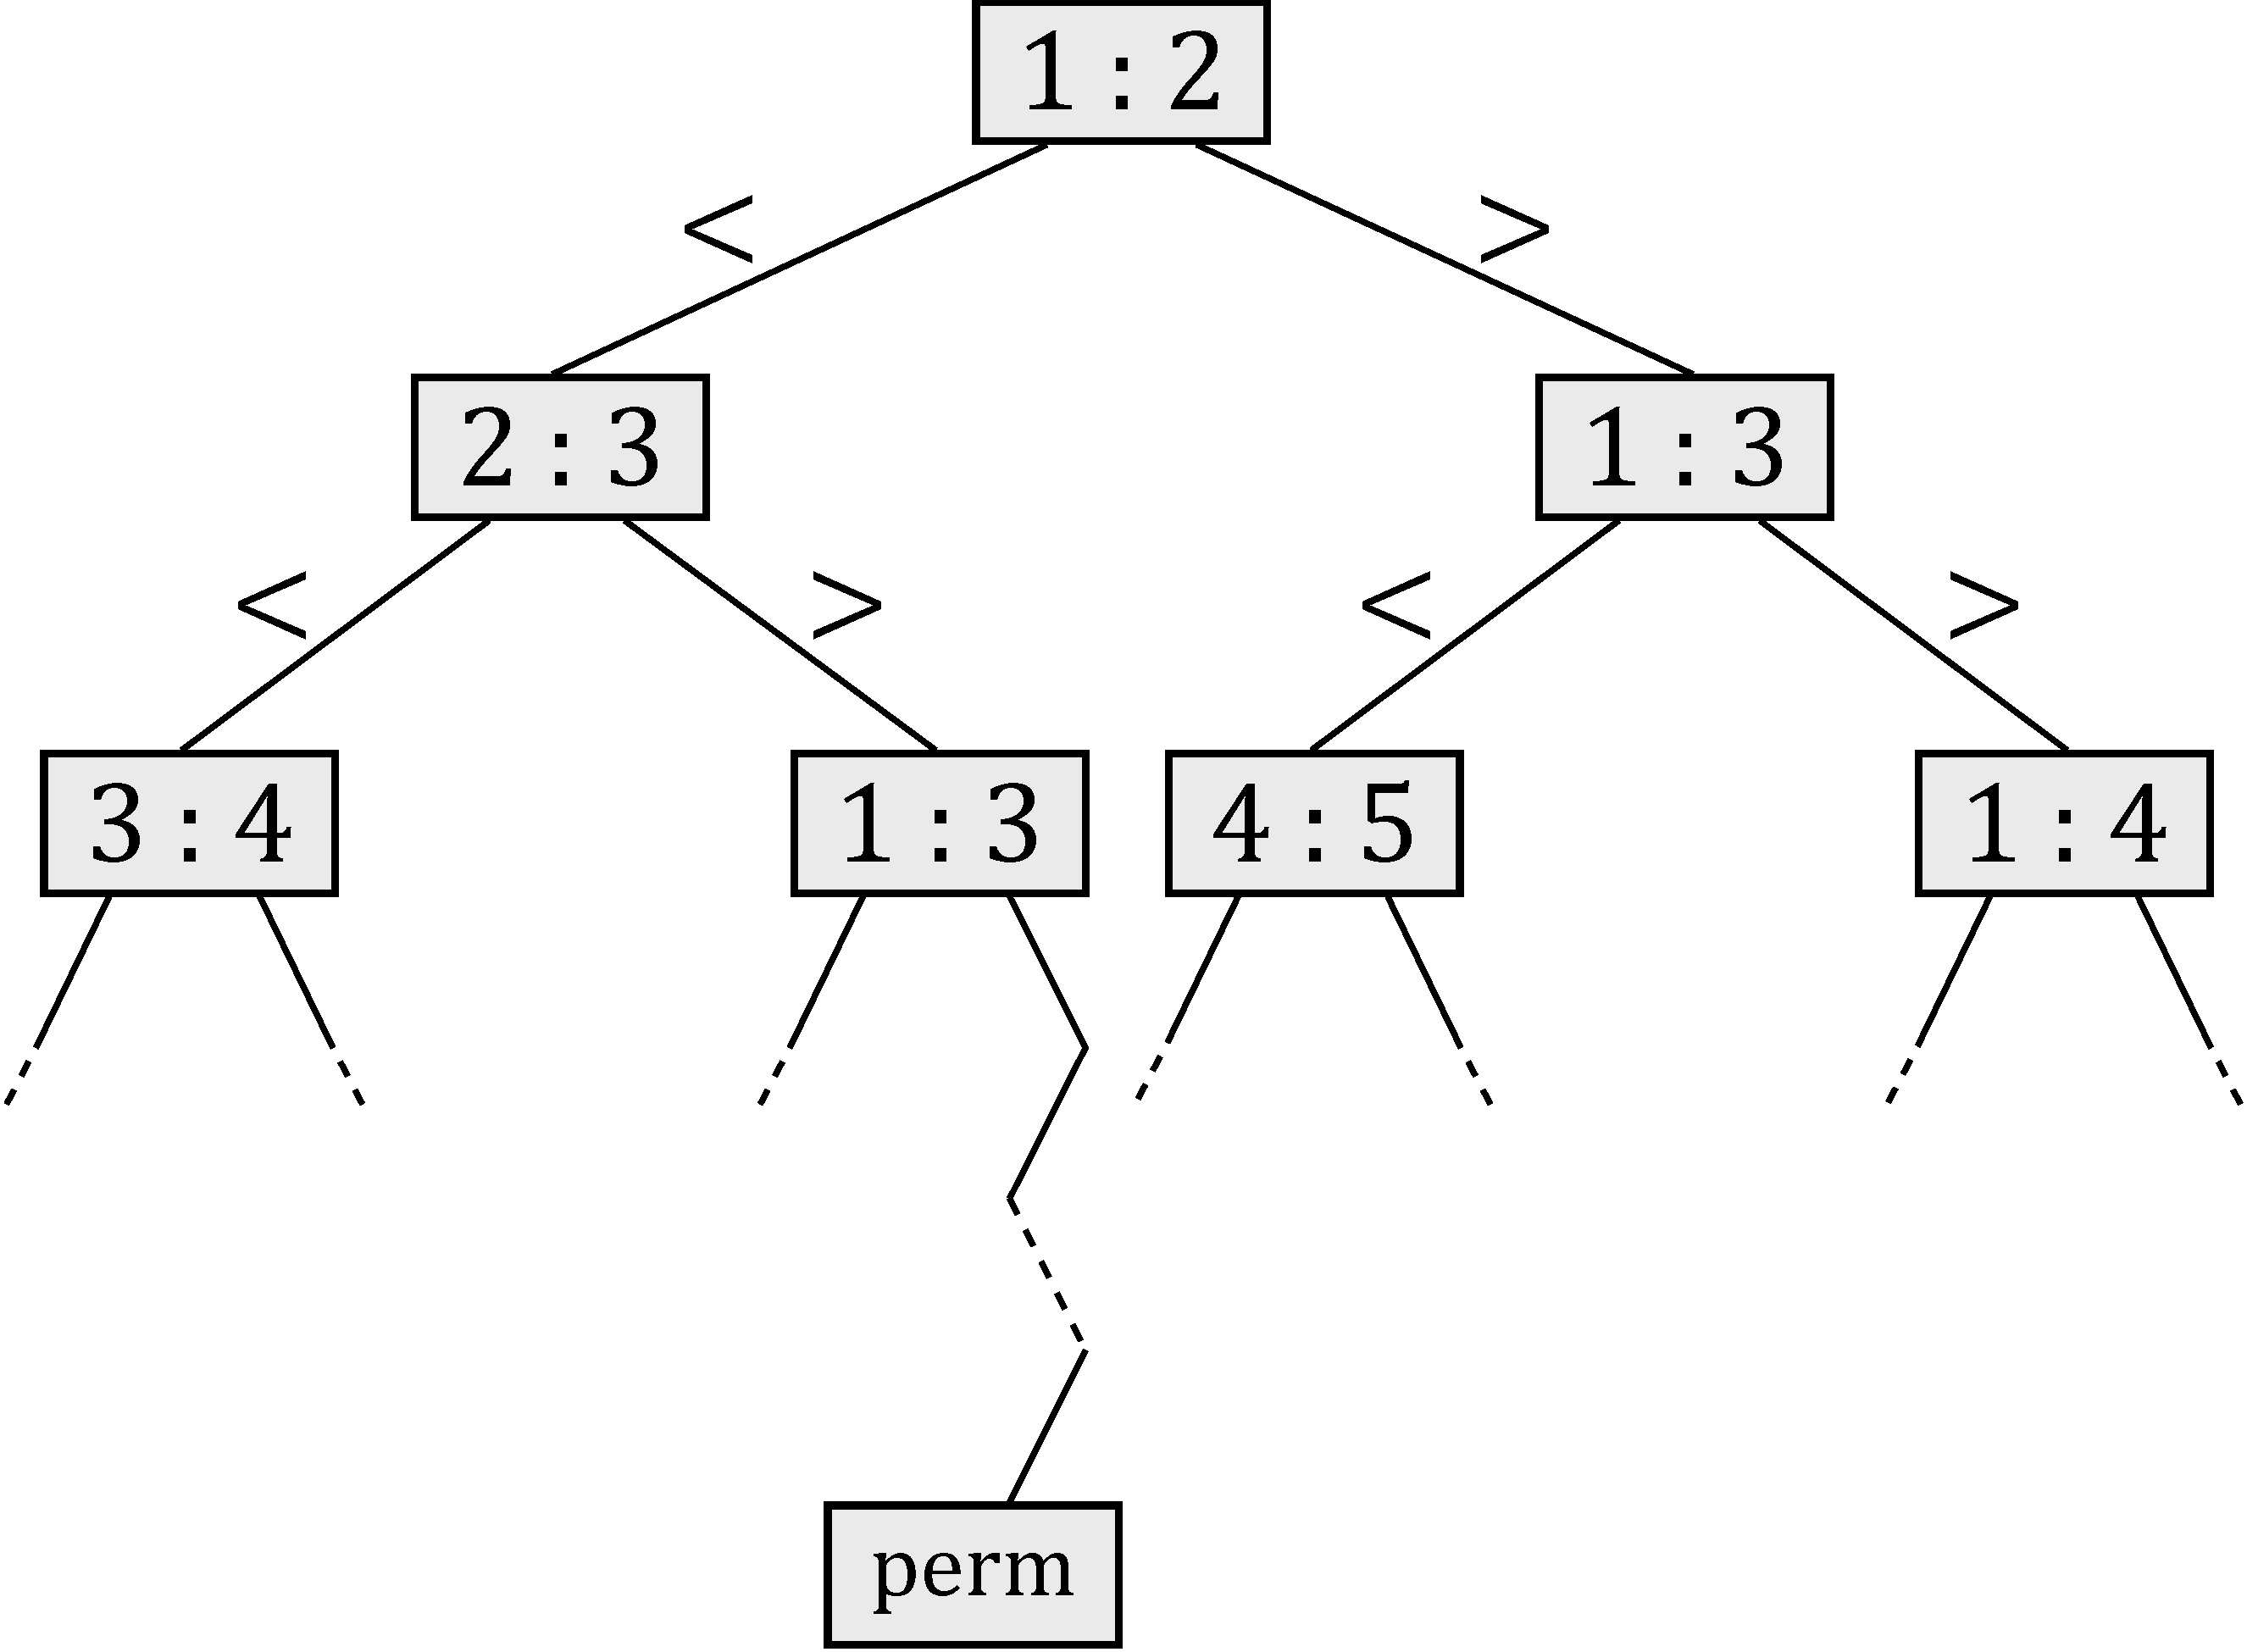
\includegraphics[width=0.6\textwidth]{beslutningstraa.pdf}
	\end{center}
	%\caption{Lower}
	\label{fig:lower}
\end{figure}

Lad nu antallet af blade være $b$ og højden $h$. Såfremt træet er perfekt balanceret kan vi presse $2^h$ blade ind i træet. Og vi ved også, at alle permutationer forekommer i bladene, derfor må $b \geq n!$ for ellers ville der ikke være plads til alle permutationer i bladene. Derfor får vi:
$$
2^h \geq b \geq n!
$$

Vi kan tage 2tals-logaritmen hvorved vi får:
$$
h \geq \lg(n!) = \Omega(n \lg n)
$$

Herved har vi altså bevist, at der er et input af længde $n$ som kræver at der bliver foretaget $h = \Omega(n \lg n)$ sammenligner.



\end{itemize}
\end{document}